% \begin{frame}{}
% Il progetto si divide in:
% \vfill
% \note{Il progetto che è stato realizzato in questo tirocinio si compone di due parti, tra loro attualmente indipendenti ma integrabili successivamente. Ossia:}

% \begin{columns}
% \begin{column}{0.48\linewidth}
% \begin{itemize}
%     \vfill
%     \item Analisi \textbf{statica}
%     \begin{itemize}
%         \item Varie tipologie di analisi
%         \item Parsing e aggregazione
%         \item Deploy in cloud su AWS
%     \end{itemize}
%     \note{
%     Uno strumento in cloud di analisi statica; che sfrutta vari tool, molto diversi tra loro, in maniera aggregata per ottenere un unico risultato finale;
%     }
%     \Pause
% \end{itemize}
% \end{column}

% \begin{column}{0.48\linewidth}
% \begin{itemize}
%     \vfill
%     \item Analisi \textbf{dinamica}
%     \begin{itemize}
%         \item Sandbox
%         \item Hardening
%         \item Sviluppo di plugin custom
%     \end{itemize}
%     \note{E poi una seconda sezione dedicata all'analisi dinamica, quindi la realizzazione, configurazione ed estensione di una sandbox al fine di fare behavioural analysis}
% \end{itemize}
% \end{column}
% \end{columns}
% \end{frame}

\begin{frame}{}
\begin{figure}
    \centering
    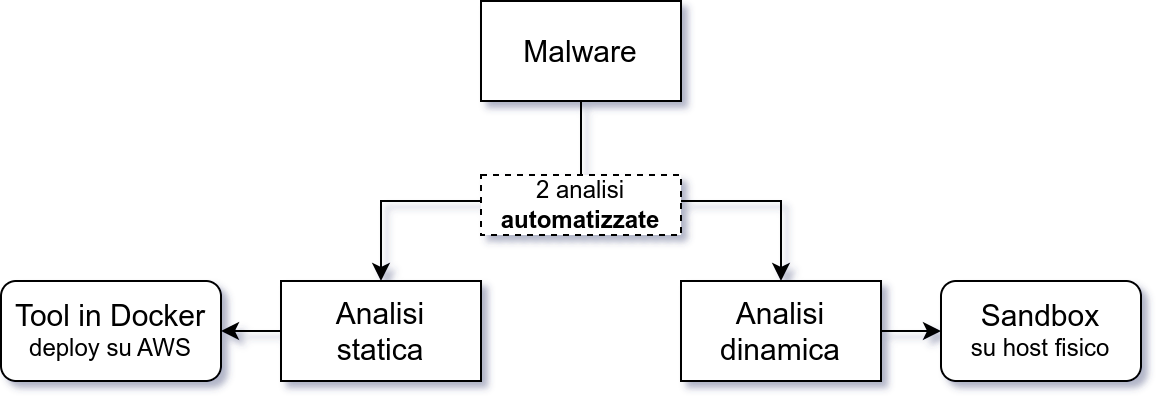
\includegraphics[width=\textwidth]{images/riepilogo_iniziale.drawio.png}
    \caption{Struttura del progetto ad alto livello}
    \label{fig:riepilogo_iniziale}
\end{figure}
\note{
Si compone di due aree:
\begin{itemize}
    \item Statica
    \begin{itemize}
        \item Dove vengono aggregati e ottimizzati vari tool molto diversi tra loro
        \item Eseguito in ambiente sicuro containerizzato
        \item Deploy dello strumento in cloud su AWS
    \end{itemize}

    \item Dinamica
    \begin{itemize}
        \item Dove viene configurata una sandbox
        \item Adeguamente isolata
        \item Estesa
        \item Resa facilmente portabile su altri sistemi
    \end{itemize}
\end{itemize}
}
\end{frame}